\section{Scaling Reasoning with Test-Time Compute}

\begin{frame}{}
    \LARGE Advanced Reasoning: \textbf{Test-Time Compute}

    \vspace{1em}
    \normalsize If a model may think for longer, how much does it gain, and what decides the limit?
\end{frame}

\begin{frame}{Why Intermediate Tokens Help, and Four Ways to Spend Them}
    \begin{itemize}\itemsep0.3em
        \item \textbf{Theory.} A constant-size transformer can solve any problem solvable by a boolean circuit of size $T$ by generating $O(T)$ intermediate tokens. Tokens buy \emph{serial computation}.
        \item \textbf{The catch.} Errors compound. With a per-step error $\epsilon$, a chain of $T$ steps is right with probability $(1-\epsilon)^T$. For $\epsilon=0.01$ and $T=128$ that is 0.276.
        \item So a long generation needs \emph{checking}. A meta-generator $y\sim\mathcal{G}(y\mid x,\,g_1,\dots,g_G,\phi)$ wraps one or more generators $g_i$ in a strategy:
    \end{itemize}
    \begin{center}
    \small
    \begin{adjustbox}{max width=\linewidth}\begin{tabular}{lll}
        \toprule
        \textbf{Pattern} & \textbf{Examples} & \textbf{What it adds} \\
        \midrule
        Chained & chain-of-thought, decomposition & depth, but no exploration of the output space \\
        Parallel & best-of-N, voting & width \\
        Tree search & beam search, REBASE, MCTS & width, guided step by step \\
        Refinement & self-correction, trained correctors & depth, guided by feedback \\
        \bottomrule
    \end{tabular}\end{adjustbox}
    \end{center}
    \src{Li et al. (ICLR 2024), as presented in Zhou, ``LLM Reasoning,'' Stanford CS25 (Apr 2025). Welleck, CMU 11-711 ``Decoding Algorithms'' (Sep 2025). Welleck et al., ``From Decoding to Meta-Generation,'' \href{https://arxiv.org/abs/2406.16838}{arXiv:2406.16838}, and NeurIPS 2024 tutorial slides.}
\end{frame}

\begin{frame}{Coverage Is Not Accuracy}
    \begin{itemize}\itemsep0.35em
        \item Sample $k$ answers. \textbf{Coverage} is the chance that at least one is right. With $C_i$ correct among $N$ samples of problem $i$:
        \[
            \text{pass@}k=\frac{1}{\#\text{problems}}\sum_i\left[1-\binom{N-C_i}{k}\Big/\binom{N}{k}\right], \qquad c(k)\approx \exp\!\big(a\,k^{b}\big)
        \]
        \item Coverage grows roughly \textbf{log-linearly over four orders of magnitude}.
        \begin{itemize}\itemsep0.15em
            \item SWE-bench Lite, DeepSeek-Coder-V2: 15.9\% with 1 sample, \textbf{56\% with 250}. Single-sample state of the art then: 43\%.
        \end{itemize}
        \item \alert{The selection gap.} Without an automatic verifier, majority voting and reward models plateau after a few hundred samples.
    \end{itemize}
    \vspace{0.1em}
    \takeaway{\textbf{2026, open-ended domains} (medicine, law, writing): ``the candidate pool is not the bottleneck, choosing from it is.'' Reward models correlate with true quality at only $\rho\approx0.12$.}
    \src{Brown et al., ``Large Language Monkeys,'' \href{https://arxiv.org/abs/2407.21787}{arXiv:2407.21787}. Romano et al., ``Test-Time Scaling in the Wild,'' \href{https://arxiv.org/abs/2608.18931}{arXiv:2608.18931}.}
\end{frame}

\begin{frame}{How Should a Budget Be Spent? It Depends on Difficulty}
    \begin{columns}[T,onlytextwidth]
        \column{0.44\textwidth}
        \centering
        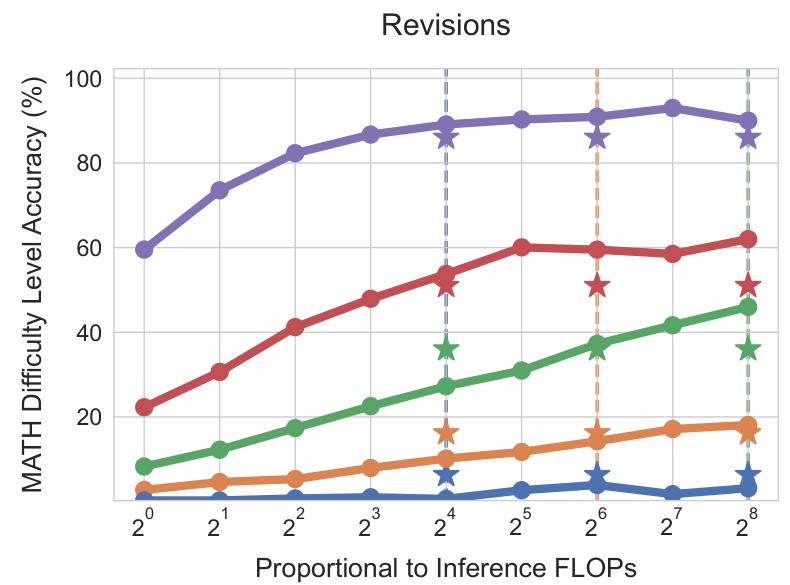
\includegraphics[width=\linewidth,height=0.54\textheight,keepaspectratio]{images/advanced-reasoning/snell_fig9_revisions_panel.png}

        {\scriptsize Lines: a small model with more inference compute, from easiest (top) to hardest questions. Stars: a larger pre-trained model.}
        \column{0.54\textwidth}
        \begin{itemize}\itemsep0.45em
            \item \textbf{Compute-optimal strategy:} per question, pick the method and settings that maximise expected accuracy for the budget. It matches best-of-N with about \textbf{4$\times$ less compute}.
            \item Easy questions prefer sequential revision, harder ones a mix with parallel search. On the hardest bin nothing helps.
            \item \textbf{Against parameters.} Let $R$ be inference tokens over pre-training tokens. If $R\ll1$, test-time compute wins on easy and medium questions. If $R\gg1$, pre-train more.
        \end{itemize}
    \end{columns}
    \vspace{0.2em}
    \caveat{``Beats a 14$\times$ larger model'' holds only where the small model already has non-trivial success.}
    \src{Snell et al., ``Scaling LLM Test-Time Compute Optimally can be More Effective than Scaling Model Parameters,'' \href{https://arxiv.org/abs/2408.03314}{arXiv:2408.03314}, Figure 9 (left panel).}
\end{frame}

\begin{frame}{Inference Has Its Own Scaling Laws}
    \begin{itemize}\itemsep0.55em
        \item \textbf{Small models can be compute-optimal.} Llemma-7B with tree search consistently beats Llemma-34B on MATH. Larger models win only after smaller ones saturate.
        \item \textbf{Voting saturates, provably.} Majority and weighted voting converge exponentially fast to a limit fixed by the model's answer distribution. More samples cannot pass it.
        \item \textbf{No strategy dominates.} A replication over 30B generated tokens, 8 open models and 4 datasets finds no single best test-time strategy.
        \item \textbf{2026: training and inference are one budget.} Train-to-Test laws optimise model size, training tokens and inference samples together. Once inference cost is counted, the optimum shifts ``radically into the overtraining regime''.
    \end{itemize}
    \vspace{0.2em}
    \takeaway{Three steps. Chinchilla optimises training FLOPs. Wu et al. optimise inference FLOPs for a given model. Train-to-Test optimises both, and lands on yesterday's over-trained small models.}
    \src{Wu et al., ``Inference Scaling Laws,'' \href{https://arxiv.org/abs/2408.00724}{arXiv:2408.00724}. Agarwal et al., ``The Art of Scaling Test-Time Compute for LLMs,'' \href{https://arxiv.org/abs/2512.02008}{arXiv:2512.02008}. Roberts et al., ``Test-Time Scaling Makes Overtraining Compute-Optimal,'' \href{https://arxiv.org/abs/2604.01411}{arXiv:2604.01411}.}
\end{frame}

\begin{frame}{Reinforcement Learning Makes Long Chains Productive}
    \begin{columns}[T,onlytextwidth]
        \column{0.46\textwidth}
        \centering
        \begin{adjustbox}{max width=\linewidth}\begin{tikzpicture}
            \begin{axis}[ybar, width=7.0cm, height=5.4cm, bar width=0.34cm,
                ymin=40, ymax=105, ylabel={\scriptsize accuracy (\%), no tools},
                symbolic x coords={AIME 2024, AIME 2025, GPQA Diamond}, xtick=data,
                x tick label style={font=\scriptsize}, y tick label style={font=\scriptsize},
                nodes near coords, nodes near coords style={font=\tiny},
                legend style={font=\tiny, at={(0.5,1.02)}, anchor=south, legend columns=3, draw=none},
                axis lines=left, enlarge x limits=0.25]
                \addplot[fill=gray!35, draw=gray] coordinates {(AIME 2024,56.3) (AIME 2025,50.4) (GPQA Diamond,67.1)};
                \addplot[fill=KAUSTcyan!45, draw=KAUSTcyan!70!black] coordinates {(AIME 2024,80.4) (AIME 2025,80.0) (GPQA Diamond,73.1)};
                \addplot[fill=darkorange!60, draw=darkorange!80!black] coordinates {(AIME 2024,95.8) (AIME 2025,92.5) (GPQA Diamond,80.1)};
                \addlegendentry{low}
                \addlegendentry{medium}
                \addlegendentry{high effort}
            \end{axis}
        \end{tikzpicture}\end{adjustbox}

        {\scriptsize gpt-oss-120b at three reasoning-effort levels}
        \column{0.52\textwidth}
        \begin{itemize}\itemsep0.45em
            \item Prompting a model to think longer does little. \textbf{Training it with outcome rewards} is what makes length pay.
            \item \textbf{DeepSeek-R1-Zero:} response length rises steadily during RL, and so does the word ``wait''. AIME 2024 pass@1 climbs from 15.6\% to 77.9\%.
            \item \textbf{Kimi k1.5:} long context RL with no tree search, no value function, no process reward model. AIME 77.5.
            \item \textbf{Qwen3, Gemini 2.5, gpt-oss:} smooth gains as the thinking budget grows.
            \item Parallel scaling still stacks on top: R1-Zero reaches 86.7\% with a vote over 16.
        \end{itemize}
    \end{columns}
    \vspace{0.1em}
    \src{OpenAI, gpt-oss model card, \href{https://arxiv.org/abs/2508.10925}{arXiv:2508.10925}. DeepSeek-AI, ``DeepSeek-R1,'' \href{https://arxiv.org/abs/2501.12948}{arXiv:2501.12948} (v2 numbers). Kimi Team, ``Kimi k1.5,'' \href{https://arxiv.org/abs/2501.12599}{arXiv:2501.12599}. Qwen3 Technical Report, \href{https://arxiv.org/abs/2505.09388}{arXiv:2505.09388}.}
\end{frame}

\begin{frame}{But Longer Is Not Always Better}
    \begin{itemize}\itemsep0.45em
        \item \textbf{Within a trained model, length is a noisy signal.} For QwQ, R1 and LIMO, correct solutions are often \emph{shorter} than incorrect ones.
        \item \textbf{An inverted U.} Accuracy peaks at an optimal chain length. It grows with difficulty and \emph{shrinks} with capability.
        \item \textbf{Overthinking.} Asked ``2+3'', QwQ-32B-Preview spends 1,953\% more tokens than a conventional LLM and writes 13 solutions. The first is right in over 92\% of cases.
        \item \textbf{Attractors (2026).} 53.8\% of sequential scaling runs enter, within four iterations, a set of answers they never leave. Mixing models lowers that rate by 21.2 points.
    \end{itemize}
    \vspace{0.1em}
    \takeaway{Overthinking, and its opposite (switching thoughts too often), are two failures of one allocation problem.}
    \src{Zeng et al., \href{https://arxiv.org/abs/2502.12215}{arXiv:2502.12215}. Wu et al., ``When More is Less,'' \href{https://arxiv.org/abs/2502.07266}{arXiv:2502.07266}. Chen et al., ``Do NOT Think That Much for 2+3=?'' \href{https://arxiv.org/abs/2412.21187}{arXiv:2412.21187}. Wang et al., \href{https://arxiv.org/abs/2501.18585}{arXiv:2501.18585}. Rance et al., \href{https://arxiv.org/abs/2609.39632}{arXiv:2609.39632}.}
\end{frame}

\begin{frame}{Controlling the Budget: From Forcing to Training}
    \begin{columns}[T,onlytextwidth]
        \column{0.4\textwidth}
        \centering
        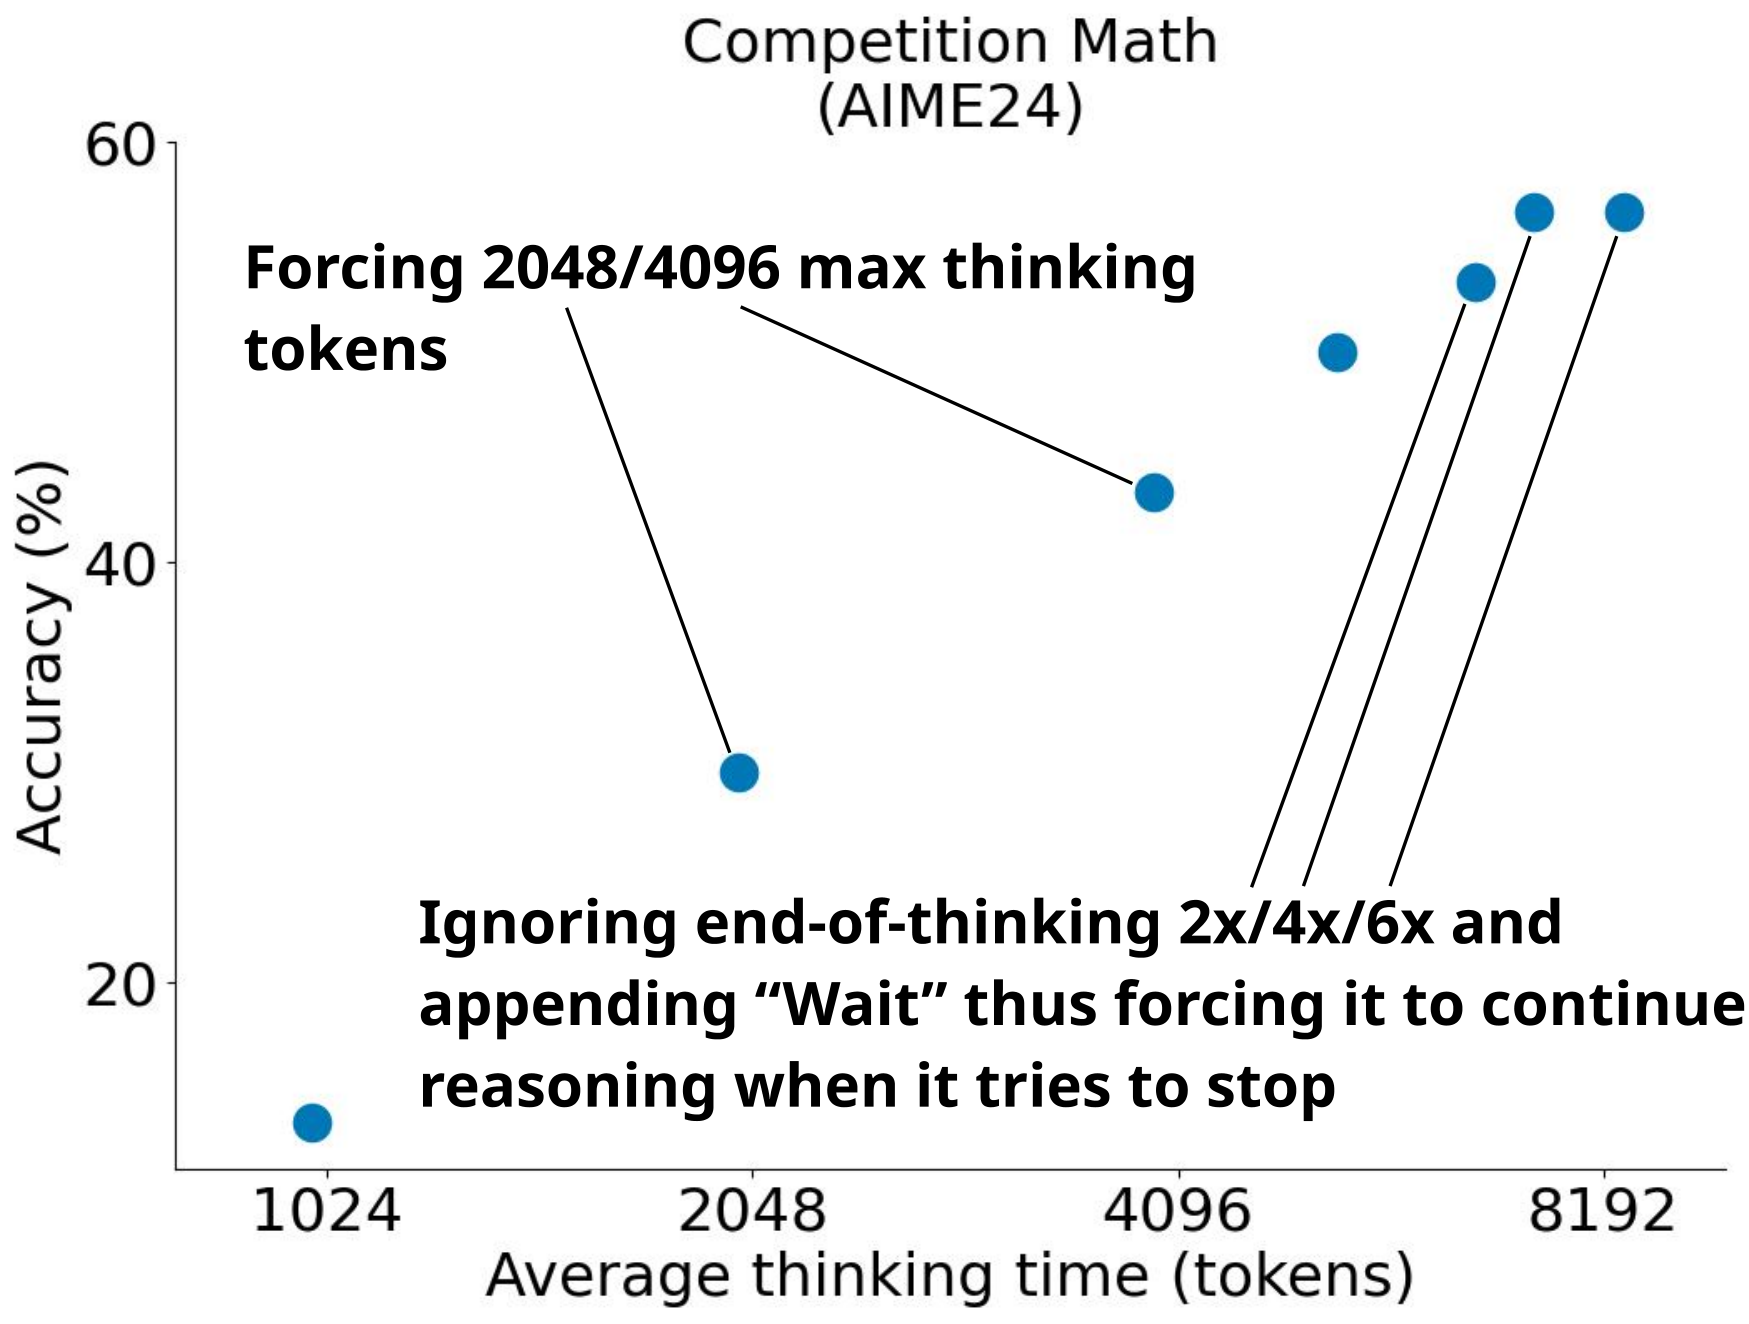
\includegraphics[width=\linewidth,height=0.6\textheight,keepaspectratio]{images/advanced-reasoning/s1_budget_forcing.png}
        \column{0.58\textwidth}
        \begin{itemize}\itemsep0.4em
            \item \textbf{s1: budget forcing at decode time.} To cap thinking, append the end-of-thinking delimiter. To extend it, suppress the delimiter and append ``Wait''.
            \begin{itemize}\itemsep0.1em
                \item AIME24 rises from 50\% to 57\%, then ``eventually flattens out''.
            \end{itemize}
            \item \textbf{L1: train the length in.} The prompt says ``Think for $N$ tokens'', and the reward penalises missing it:
            \[
                r=\mathbb{1}(y=y_{\text{gold}})-\alpha\,|n_{\text{gold}}-n_y|
            \]
            \begin{itemize}\itemsep0.1em
                \item 20 to 25 points above budget forcing at equal length. Mean length error about 3\%.
            \end{itemize}
            \item Trained control beats decode-time intervention. Production systems took the same road.
        \end{itemize}
    \end{columns}
    \vspace{0.1em}
    \src{Muennighoff et al., ``s1: Simple test-time scaling,'' \href{https://arxiv.org/abs/2501.19393}{arXiv:2501.19393}, Figure 1. Aggarwal and Welleck, ``L1: Controlling How Long A Reasoning Model Thinks With RL,'' \href{https://arxiv.org/abs/2503.04697}{arXiv:2503.04697}.}
\end{frame}

\begin{frame}{From Token Budgets to Effort Dials (October 2026)}
    \begin{center}
    \small
    \renewcommand{\arraystretch}{1.15}
    \begin{adjustbox}{max width=\linewidth}\begin{tabular}{>{\raggedright\arraybackslash}p{2.3cm}>{\raggedright\arraybackslash}p{5.3cm}>{\raggedright\arraybackslash}p{6.2cm}}
        \toprule
        \textbf{Provider} & \textbf{Control} & \textbf{Note} \\
        \midrule
        Anthropic & adaptive thinking plus effort: low to max & token budgets are rejected on Claude 4.7 and later \\
        OpenAI & \texttt{reasoning.effort}: none to max & reasoning tokens are hidden but billed as output \\
        Google & \texttt{thinking\_level}: minimal to high & thought tokens count against the output limit \\
        xAI & effort: low to xhigh & cannot be switched off. On the multi-agent model, effort sets \emph{how many agents collaborate} \\
        Open weights & Qwen3 \texttt{/think}, gpt-oss ``Reasoning: low'' & DeepSeek-V4.1-Flash: effort from 1 to 100 \\
        \bottomrule
    \end{tabular}\end{adjustbox}
    \end{center}
    \begin{itemize}\itemsep0.3em
        \item Three generations of control: decode-time forcing, trained length conditioning, then a \textbf{coarse dial with the model deciding} how much to think.
    \end{itemize}
    \src{Anthropic, extended thinking and effort documentation. OpenAI, reasoning models guide. Google, Gemini API thinking documentation. xAI, reasoning guide. Qwen3 blog (Apr 2025). DeepSeek-V4.1-Flash release note (Sep 2026). All accessed 3 Oct 2026.}
\end{frame}

\begin{frame}{When More Thinking Hurts}
    \centering
    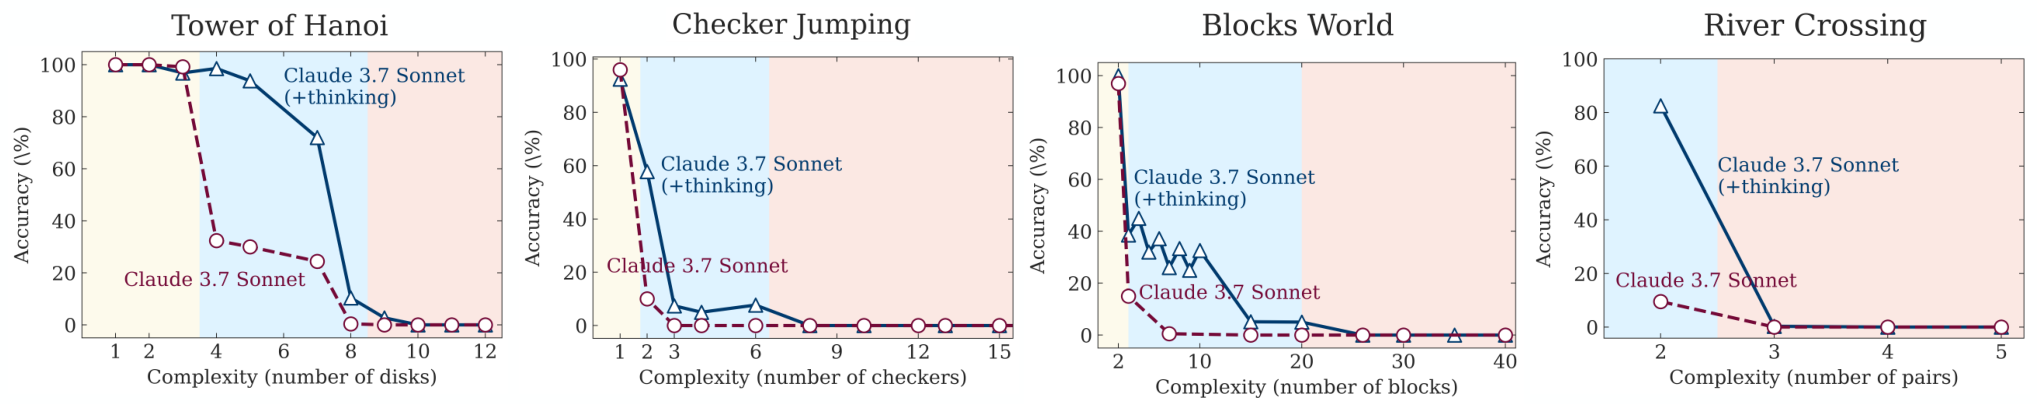
\includegraphics[width=0.98\linewidth,height=0.34\textheight,keepaspectratio]{images/advanced-reasoning/illusion_three_regimes_claude.png}
    \begin{itemize}\itemsep0.3em
        \item \textbf{``The Illusion of Thinking'':} three regimes on puzzles. Easy: thinking is wasted. Medium: it helps. Hard: both variants collapse.
        \item \textbf{The rebuttal:} move lists exceed the output limit, and some instances are impossible.
        \item \textbf{Inverse scaling:} with longer reasoning, nine models get worse on some tasks.
        \item \textbf{Knowledge tasks:} more thinking often adds hallucinations. It cannot add facts.
    \end{itemize}
    \src{Figure: Shojaee et al. (Apple), \href{https://arxiv.org/abs/2506.06941}{arXiv:2506.06941}. Lawsen, \href{https://arxiv.org/abs/2506.09250}{arXiv:2506.09250}. Dellibarda Varela et al., \href{https://arxiv.org/abs/2507.01231}{arXiv:2507.01231}. Gema, H\"agele et al., \href{https://arxiv.org/abs/2507.14417}{arXiv:2507.14417}. Knowledge tasks: \href{https://arxiv.org/abs/2509.06861}{arXiv:2509.06861}.}
\end{frame}

\begin{frame}{Test-Time Compute: What to Remember}
    \begin{itemize}\itemsep0.6em
        \item Test-time compute is \textbf{generation plus selection}. Coverage is the upper bound. The verifier decides how much of it you keep.
        \item Gains are \textbf{log-linear}, depend on difficulty, and are bounded by the base model.
        \item \textbf{Outcome-reward RL} is what turned longer chains into better answers. Within a trained model, length alone is a noisy signal.
        \item The interface settled on \textbf{effort dials}. The research question moved from ``does it scale?'' to ``how do we allocate, verify and bound it?''
    \end{itemize}
    \vspace{0.3em}
    \vspace{0.3em}
    \takeaway{\textbf{Next.} Tokens can be spent in one chain, many chains, a tree or a graph. Which structure, and does the choice still matter?}
\end{frame}
